\documentclass{standalone}
\usepackage{pgfplots}
\pgfplotsset{compat=1.18} % Set to the latest version of pgfplots
\usepgfplotslibrary{external}
\usepgfplotslibrary{units}
\usepackage{amsmath}
\usepackage{xcolor}
%%%%%%%%%%%%%%%%%%%%%%%%%%%%
% Rose Pine 
%%%%%%%%%%%%%%%%%%%%%%%%%%%%
\definecolor{base}{HTML}{191724}
\definecolor{surface}{HTML}{1f1d2e}
\definecolor{overlay}{HTML}{26233a}
\definecolor{muted}{HTML}{6e6a86}
\definecolor{subtle}{HTML}{908caa}
\definecolor{text}{HTML}{e0def4}
\definecolor{love}{HTML}{eb6f92}
\definecolor{gold}{HTML}{f6c177}
\definecolor{rose}{HTML}{ebbcba}
\definecolor{pine}{HTML}{31748f}
\definecolor{foam}{HTML}{9ccfd8}
\definecolor{iris}{HTML}{c4a7e7}


\begin{document}

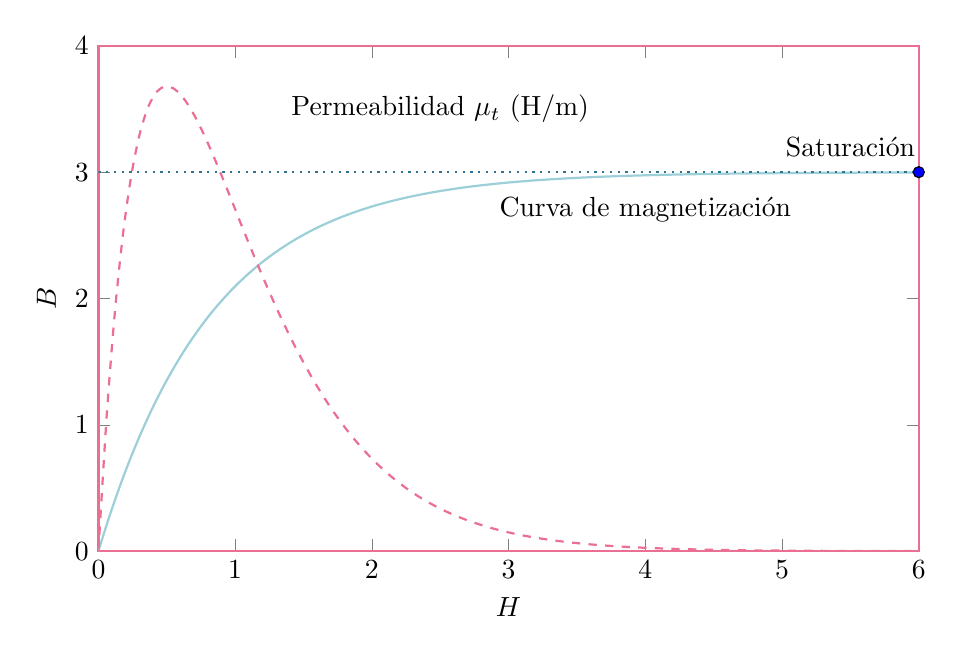
\begin{tikzpicture}
    \begin{axis}[
        width=12cm, height=8cm,
        xlabel={$H$},
        ylabel={$B$},
        xmin=0, xmax=6,
        ymin=0, ymax=4, % Set ymax closer to 4
        xtick={0,1,...,6},
        ytick={0,1,...,4},
        enlargelimits=false,
        grid=none, % Remove grid lines
        axis line style={draw=love,thick}, % Change 'love' to your desired axis color
    ]

    % Magnetization curve (solid green)
    \addplot [
        thick,
        smooth,
        domain=0:6,
        samples=100,
        color=foam
    ]
    {3 * (1 - exp(-1.2*x))}; % Exponential growth towards saturation

    % Permeability curve (dashed red)
    \addplot [
        thick,
        dashed,
        smooth,
        domain=0:6,
        samples=100,
        color=love
    ]
    {20 * x * exp(-2*x)}; % Increased the multiplier to 20 to raise the peak, with fast decay

    % Adding the annotations
    \node at (axis cs:4,2.7) {Curva de magnetización};
    \node at (axis cs:2.5,3.5) {Permeabilidad $\mu_t$ (H/m)};
    
    % Marking the saturation point
    \addplot[only marks, mark=*, mark options={fill=blue}] coordinates {(6, 3)};
    \node at (axis cs:5.5,3.2) {Saturación};
 \addplot [
        thick,dotted,
        color=pine,
        domain=0:6
    ]
    {3}; % Y value at the saturation point

    \end{axis}

\end{tikzpicture}

\end{document}
